\documentclass{article}
\usepackage[english]{babel}
\usepackage{graphicx,times,amsmath,colortbl, psfrag,listings}
\usepackage[ruled, vlined, english, boxed, linesnumbered, lined]{algorithm2e}
\usepackage[letterpaper,top=2cm,bottom=2cm,left=3cm,right=3cm,marginparwidth=1.75cm]{geometry}
\usepackage{amsmath}
\usepackage{listings}
\usepackage{algorithm}
\usepackage{algorithmic}
\usepackage{algpseudocode}
\usepackage{graphicx}
\usepackage[colorlinks=true, allcolors=blue]{hyperref}
\usepackage{algpseudocode} 
\usepackage{multirow}
\graphicspath{ {/} }
\usepackage {amsfonts}
\begin{document}
\begin{titlepage}
\centering

{\bfseries\LARGE Instituto Polit\'ecnico Nacional \par}
\vspace{1cm}
{\scshape\Large Escuela Superiror de Computaci\'on \par}
\vspace{3cm}
{\scshape\Huge  AJEDREZ \par}
\vspace{3cm}
{\itshape\Large Pr\'actica 5 \par}
\vfill
{\Large Alumno: \par}
{\Large Alcántara Covarrubias Erik \par}
{\Large Profesor: \par}
{\Large Juarez Martinez Genaro \par}
{\Large Grupo: 4CM6\par}
\vfill
\end{titlepage}
\section{Introducci\'on}
Un autómata finito no determinístico es aquel que puede estar en varios estados a la vez, al igual que un autómata finito determinístico tiene un conjunto finito de estados, un conjunto finito de símbolos de entrada, un estado inicial y un conjunto de estados finales. También tiene funciones de transición. \newline \newline
Un autómata finito no determinístico se representa esencialmente como un autómata finito determinístico:
\begin{equation}
A =\{Q,\sum,\delta,q_0,F\}
\end{equation}
donde:
\begin{itemize}
    \item $Q$ es un conjunto finito de estados.
    \item $\sum$ es un conjuto finito de símbolos de entrada.
    \item $q_0$, un elemento de $Q$, es el estado inicial.
    \item $F$, un subconjunto de $Q$, es el conjunto de estados finales (o de aceptación).
    \item $\delta$ la función de transición, es una función que toma como argumentos un estado de $Q$ y un símbolo de entra de $\sum$ y devuelve un subconjunto de $Q$. Observe que la única diferencia entre un AFN y un AFD se encuentra en el tipo de calor que devuelve $\delta$: un conjunto de estados en el caso de un AFN y un único estado en el caso de un AFD. 
\end{itemize}
\section{Marco teórico}
Primero denominaremos el tablero junto con la numeración que se le tiene que dar, para las rutas el uso de los números es lo principal al igual que los colores de las casillas, cuando se tiene esto se puede usar un AFN para darnos una idea de como generarlas.Las entradas del programa pide las rutas por medio de colores, las rutas numéricas se calculan de manera aleatoria.
Ya teniendo el AFN, las reglas para poder construir el AFD desde el AFN son los siguientes:
\begin{itemize}
    \item Si $q_0$ es el estado inicial del AFN, entonces \{$q_0$\} es uno de los estados del AFD.
    \item Suponemos que $p$ es uno de los estados del AFN y se llega a él desde el estado inicial siguiendo un camino cuyos símbolos son $a_1a_2...a_m$. Luego uno de los estados del AFD es el conjunto de estados del AFN constituidos por:
    \begin{itemize}
        \item $q0$.
        \item $p$.
        \item Cualquier otro estado del AFN al que se pueda llegar desde $q_0$ siguiendo un camino cuyas etiquetas sean un sufijo de $a_1a_2...a_m$ es decir, cualquier secuencia de símbolos de la forma $a_ja_{j+1}...a_m$.
    \end{itemize}
\end{itemize}
\section{Explicaci\'on del problema e implementaci\'on del algoritmo}
\subsection{Problema a resolver}
Elaborar un programa para realizar movimientos ortogonales y diagonales en un tablero de ajedrez de 4x4 con dos piezas. Los movimientos y las reglas están explicadas en las láminas del curso de Stanford.\newline
Adicionalmente, el programa debe de contar con las siguientes características:
\begin{enumerate}
    \item Debe de correr en modo automático (todo) y forma manual.
    \item En el caso de forma manual, el usuario podrá introducir la cadena de movimientos o generarla aleatoriamente.
    \item El programa puede correr con una pieza o dos.
    \item En el caso de dos piezas, la segunda iniciará en el estado 4 y su estado final es el estado 13.
    \item  Cuando inicie el juego, de manera aleatoria el programa debe decidir quién inicia primero.
    \item Una vez definida la cadena de movimientos para uno o dos piezas, se deben generar los archivos de todos los movimientos posibles por pieza, generar otro archivo con todos los movimientos ganadores por pieza. Estos dos últimos archivos servirán para reconfigurar las rutas.
    \item Si se reconfigura una ruta y aún así no se puede avanzar, entonces habrá que esperar una iteración para continuar.
    \item Graficar el tablero y mostrar los movimientos de una pieza o dos piezas.
    \item Si se escoge el modo automático las cadenas generadas no deben ser mayores a 10 movimientos para la animación.
    \item El número máximo de movimientos deberá de ser de a lo más 100 símbolos.
\end{enumerate}
\subsection*{Implementaci\'on}
\begin{lstlisting}

    import random
    from time import sleep
    import pygame
    
    class ficha():
        def __init__(self, image):
            self.image = image
        
        def decoder(self,route, size):
            """
            It takes a string of letters and converts them into a list of tuples
            
            :param route: The route that the player will take
            :param size: The size of the square that will be drawn
            """
            tabla_coordenadas = {
            'a' : (1*size, 1*size), 'b' : (2*size, 1*size), 'c' : (3*size, 1*size), 'd' : (4*size, 1*size),
            'e' : (1*size, 2*size), 'f' : (2*size, 2*size), 'g' : (3*size, 2*size), 'h' : (4*size, 2*size),
            'i' : (1*size, 3*size), 'j' : (2*size, 3*size), 'k' : (3*size, 3*size), 'l' : (4*size, 3*size),
            'm' : (1*size, 4*size), 'n' : (2*size, 4*size), 'o' : (3*size, 4*size), 'p' : (4*size, 4*size)
            }
            logic_route = []
            for i in route:
                logic_route.append(tabla_coordenadas.get(i))
            self.route = logic_route
    
    # A dictionary that contains the possible states that the knight can go to, depending on the current
    # state and the instruction.
    tabla_estados = {
            'a' : {'W': 'be', 'R': 'f'},
            'b' : {'W': 'eg', 'R': 'acf'},
            'c' : {'W': 'bdg', 'R': 'fh'},
            'd' : {'W': 'g', 'R': 'ch'},
            'e' : {'W': 'bj', 'R': 'afi'},
            'f' : {'W': 'ebjg', 'R': 'acik'},
            'g' : {'W': 'bdjl', 'R': 'cfik'},
            'h' : {'W': 'gdl', 'R': 'ck'},
            'i' : {'W': 'ejm', 'R': 'gn'},
            'j' : {'W': 'egmo', 'R': 'fikn'},
            'k' : {'W': 'jglm', 'R': 'fhnp'},
            'l' : {'W': 'go', 'R': 'hkp'},
            'm' : {'W': 'j', 'R': 'in'},
            'n' : {'W': 'mjo', 'R': 'ik'},
            'o' : {'W': 'jl', 'R': 'nkp'},
            'p' : {'W': 'ol', 'R': 'k'}
    }
    
    def recalculate(route_1:list, route_2:list, num_try:int, starter:int):
        """
        If there is a coincidence between the 2 routes, depending in which one started the other one
        will be recalculated, if there is again another coincidence the route will stop.
        
        :param route_1: the first route
        :param route_2: the route that is being compablack to route_1
        :param num_try: This is the number of times the algorithm has tried to find a solution
        :param starter: Who start the game
        :return: a boolean value, and the two routes.
        """
        try:
            for i in range( len(route_1) ):
                if(route_1[i]==route_2[i]):
                    if(num_try == 2):
                        if (starter == 1):
                            route_1.insert(i,route_1[i-1])
                            route_1.insert(i,route_1[i-2])
                        else:
                            route_2.insert(i,route_2[i-1])
                            route_2.insert(i,route_2[i-2])
                        return False, route_1, route_2
                    else:
                        return True, route_1, route_2
                
            return False, route_1, route_2
    
        except IndexError:
            return False, route_1, route_2
        
    def rand_start():
        """
        It takes a random number between 1 and 10. If the number is even, it returns 2, otherwise it
        returns 1.
        :return: 1 or 2.
        """
        a = random.randint(1,10)
        if(a % 2 == 0):
            return 2
        else:
            return 1
        
    def clean_routes(end, path):
        """
        It takes a path and returns the path until the first time you get to the end
        
        :param end: the end node of the path
        :param path: the path to be cleaned
        :return: the path from the start to the end.
        """
        index = path.index(end)
        return path[0:index+1]
    
    def routes(current, path):
        """
        It takes a current state and a path, and yields all the possible routes that can be taken from the
        current state to the end of the path
        
        :param current: the current state
        :param path: the path to be tested
        :return: A generator that yields all possible routes from the initial state to the final state.
        """
        if not path:
            yield (current,)
            return
        first, *newpath = path
        for state in tabla_estados[current][first]:
            for route in routes(state, newpath):
                yield (current,) + route
                """print(newpath)
                print(tuple(current)+tuple(route))"""
    
    def chess(path, inicio):
        """
        It takes a starting point and a path, and then it writes all the possible routes to a file
        
        :param path: The path of the file containing the graph
        :param inicio: The starting point of the knight
        """
        all_routes = open("Practica5/all_routes"+inicio+".txt", "w+")
        for i, W in enumerate(routes(inicio, path), 1):
            all_routes.write(''.join(W))
            all_routes.write("\n")
        print("Rutas totales encontradas: "+str(i))
    
    def randomInst(num):
        """
        It generates a random string of length num, where each character is either R or W
        
        :param num: number of instructions
        :return: A string of random characters.
        """
        aux = "";
        for i in range(num):
            a = random.randint(1,2);
            if(a % 2 == 0):
                aux = aux + "R"
            else:
                aux = aux + "W"
        return aux
    
    def best_routes(possible_routes,end):
        """
        It takes a file with all the possible routes and a letter that represents the end of the route, and
        returns the 5 best routes
        
        :param possible_routes: the file that contains all the possible routes
        :param end: The last letter of the route
        :return: the 5 best routes.
        """
        winning_routes = open("Practica5/winning_routes"+end+".txt", "w+")
        with open(possible_routes) as openfileobject:
            i=0
            rank = []
            for line in openfileobject:
                if(end in line):
                    clean_line = clean_routes(end, line)
                    winning_routes.write(line)
                    winning_routes.write("\n")
                    rank.append(clean_line)
                    i+=1
            # It removes duplicates from the list.
            clean_rank = list(dict.fromkeys(rank))
            # It sorts the list of routes by length, so the shortest route is the first element of the
            # list.
            rank_5 = sorted(clean_rank, key=lambda x: len(x))
            print("Rutas ganadoras encontradas:" + str(i))
            print("Mejores rutas: ")
            print(rank_5[-5:])
        return rank_5[-5:]
                    
    # A way to run the code only if the file is executed directly.
    if __name__ == "__main__":
        while True:
            try:
                opc = input("Todo automatico? (Y/N): ").lower
                if(opc != "n"):
                    num_jugadores = rand_start()
                    rute = randomInst(random.randint(1,10))
                
                else:    
                    num_jugadores = int(input("Cuantos jugadores vas a usar? (1,2): "))
                    if (num_jugadores < 1):
                        break
                    rute = input("Ingrese la cadena a evaluar usando R y W (si quiere random ponga 0): ").upper()
                
                    #Info gather
                    if (rute == "0"):
                        rute = randomInst(random.randint(1,10))
                
                    if (len(rute) >= 100):
                        print("Error, mas de 100 caracteres")
                        break
                
                print("Ruta a evaluar: "+rute)
                
                #Begin Calc for players
                print("Calculando rutas de ficha 1")
                chess(rute, 'a')
                routes_1=best_routes("Practica5/all_routesa.txt", 'p')
                b_piece=ficha('Practica5/B_piece.png')
                b_player = pygame.image.load(b_piece.image)
                b_player = pygame.transform.scale(b_player, [50,50])
                
                if(num_jugadores >= 2): 
                    print("Calculando rutas de ficha 2")
                    chess(rute, 'd')
                    routes_2=best_routes("Practica5/all_routesd.txt", 'm')
                    w_piece = ficha('Practica5/W_piece.png')
                    w_player = pygame.image.load(w_piece.image)
                    w_player = pygame.transform.scale(w_player, [50,50])
                
                #Refine ouputs
                try:
                    if(num_jugadores >= 2):
                        inicio = rand_start()
                        print("Inicia: "+str(inicio))
                        accept, final_r1, final_r2 = recalculate(list(routes_1[0]), list(routes_2[0]), 1, inicio)
                        if(accept):
                            if (inicio == 1):
                                accept, final_r1, final_r2 = recalculate(list(routes_1[0]), list(routes_2[1]), 2, inicio)
                            else:
                                accept, final_r1, final_r2 = recalculate(list(routes_1[1]), list(routes_2[0]), 2, inicio)
                        r1 = ''.join(final_r1)
                        r2 = ''.join(final_r2)
                        
                    else:
                        r1 = routes_1[0]
                    pygame.display.init()
                    
                    #color in rgb values
                    white,black = (245,245,220),(155,155,155)                
                    
                    #set display
                    gameDisplay = pygame.display.set_mode((600,600))
                    pygame.display.set_caption("ChessBoard")
                    
                    #beginning of logic
                    #Size of squares
                    size = 100
    
                    #board length, must be even
                    boardLength = 4
                    gameDisplay.fill(white)
    
                    cnt = 0
                    for i in range(1,boardLength+1):
                        for z in range(1,boardLength+1):
                        #check if current loop value is even
                            if cnt % 2 == 0:
                                pygame.draw.rect(gameDisplay, white,[size*z,size*i,size,size])
                            else:
                                pygame.draw.rect(gameDisplay, black, [size*z,size*i,size,size])
                            cnt +=1
                            #since theres an even number of squares go back one value
                        cnt-=1
                        #Add a nice boarder
                   
                    pygame.draw.rect(gameDisplay,black,[size,size,boardLength*size,boardLength*size],1)
                    gameDisplay.blit(b_player,[size,size])
                    b_piece.decoder(r1, size)
                    
                    if (num_jugadores >= 2):
                        gameDisplay.blit(w_player,[4*size, size])
                        w_piece.decoder(r2, size)
                    
                    #print the pieces
                    pygame.display.update()
                    
                    if (num_jugadores >= 2):
                        if(len(b_piece.route) > len(w_piece.route)):
                            movements = len(w_piece.route)
                        else:
                            movements = len(b_piece.route)
                        
                        try:
                            if(inicio == 1):
                                for i in range(movements):
                                    gameDisplay.blit(b_player,list(b_piece.route[i]))
                                    pygame.display.update()
                                    sleep(3)
                                    gameDisplay.blit(w_player,list(w_piece.route[i]))
                                    pygame.display.update()
                                    sleep(3)
                            else:
                                for i in range(movements):
                                    gameDisplay.blit(w_player,list(w_piece.route[i]))
                                    pygame.display.update()
                                    sleep(3)
                                    gameDisplay.blit(b_player,list(b_piece.route[i]))
                                    pygame.display.update()
                                    sleep(3) 
                            print("Termino la partida")
                            sleep(10)
                            pygame.display.quit()
                        
                        except IndexError:
                            print("Termino la partida")
                            sleep(10)
                            pygame.display.quit()
                    
                    else:
                        for i in b_piece.route:
                            gameDisplay.blit(b_player,list(i))
                            pygame.display.update()
                            sleep(3)
                        print("Termino la partida")
                        sleep(10)
                        pygame.display.quit()
                
                except IndexError:
                    print("No hay rutas ganadoras para 1 o mas jugadores")
                
                opc = input("Salir? (Y/N): ").lower()
                tab = []
                if (opc != "n"):
                    print("\nAdios!!")
                    pygame.display.quit()
                    quit()
                    
            except KeyboardInterrupt:
                print("\nAdios!!")
                pygame.display.quit()
                quit()
                
            except KeyError:
                print("La cadena tiene caracteres no validos, favor de revisar")
            
            except ValueError:
                print("Valor incorrecto")
                pass
\end{lstlisting}

\subsection*{Capturas de Resultados}
\begin{center}
    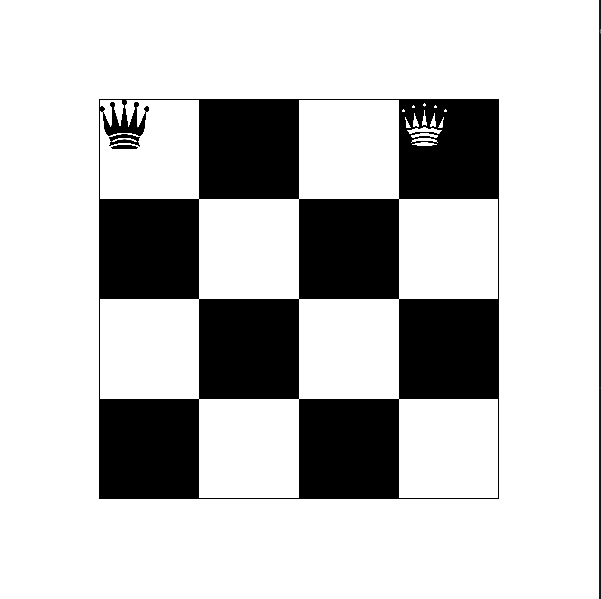
\includegraphics[width=\textwidth]{Practica7-capt1.png}
    Primer prototipo del tablero
    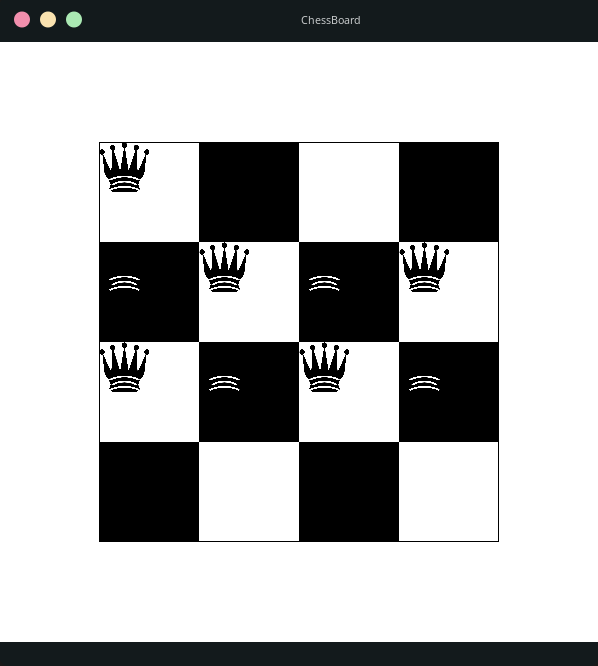
\includegraphics[width=\textwidth]{Practica7-capt2.png}
    Movimientos de ficha
    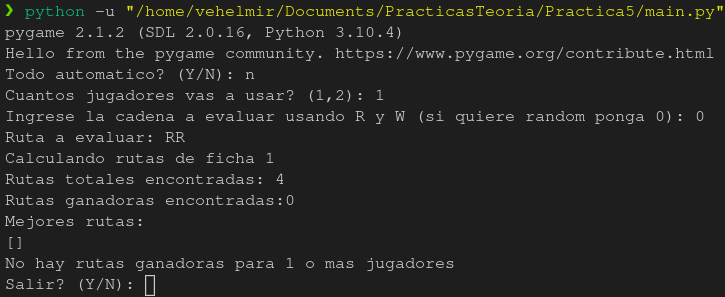
\includegraphics[width=\textwidth]{Practica7-capt3.png}
    Salidas en consola de una ejecucion normal sin ruta ganadora
    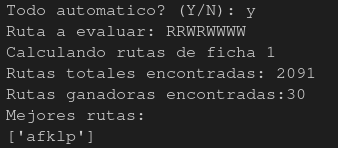
\includegraphics[width=\textwidth]{Practica7-capt4.png}
    Salida en consola de una ruta que puede ganar
    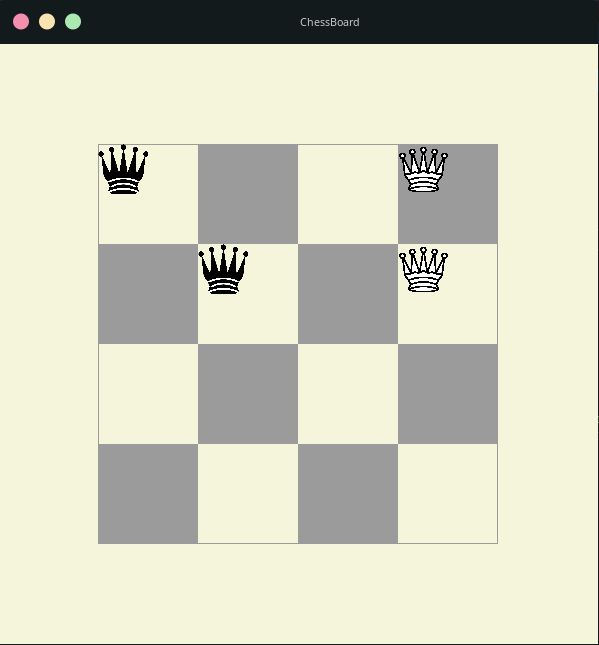
\includegraphics[width=\textwidth]{Practica7-capt5.png}
    Tablero Final, Mejora de colores
    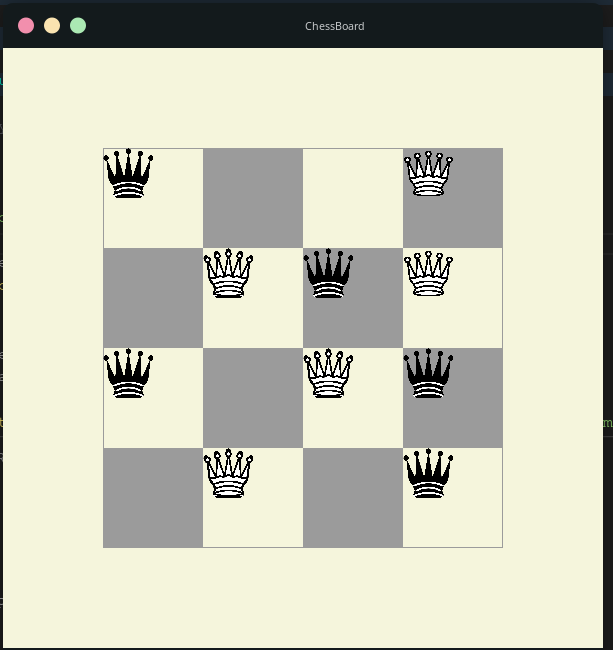
\includegraphics[width=\textwidth]{Practica7-capt6.png}
    Tablero con una partida representada
    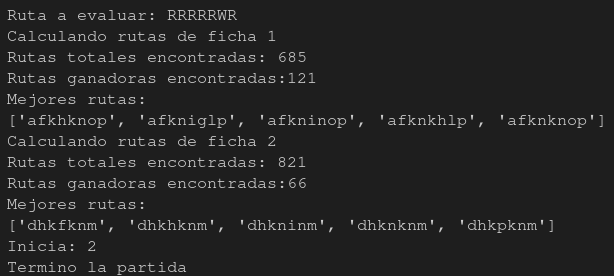
\includegraphics[width=\textwidth]{Practica7-capt7.png}
    Salida en consola de todos los calculos que se hicieron
\end{center}
Se crean 4 archivos .txt, 1 de cada tipo por ficha:
\begin{itemize}
    \item $all\_routes*.txt$: Que muestra todas las rutas posibles para una instruccion.
    \item $winning\_routes*.txt$: Las rutas ganadoras.
\end{itemize}
\section*{Conclusi\'on}

\section*{Bibliograf\'ia}
\begin{itemize}
    \item Introduction to Automata Theory, Languages, and Computation
    John E. Hopcroft, Rajeev Motwani, Jeffrey D. Ullman
    Pearson/Addison Wesley, 2nd edition
    \item Software Foundation, P. (2022, 13 enero). 3.10.2 Documentation. Documentación de Python. Recuperado 15 de febrero de 2022, de https://docs.python.org/es/3/
\end{itemize}
\end{document}
